%!TEX root = ../thesis.tex
%*******************************************************************************
%****************************** Second Chapter *********************************
%*******************************************************************************

\chapter{The LHC and the CMS Experiment}

\section{The Large Hadron Collider}

The LHC \cite{1748-0221-3-08-S08001} is a circular proton proton accelerator with a circumference of $27 \; \mathrm{km}$ that is designed for a collision energy of $\sqrt{s} = 14 \; \TeV$.
This analysis uses data of proton proton collisions taken in 2016 where the LHC reached a center of mass energy of $\sqrt{s}= 13 \; \TeV$.
The protons are assembled in bunches and accelerated to an energy of  $450 \; \GeV$ by various pre-accelerators before being injected into the LHC.
The two beams in the LHC run in opposite directions and are led by 2136 superconducting dipole magnets.

Colissions are induced at four points along the ring of the LHC. The four main experiments are situated at these interaction points.
The ALICE (A Large Ion Collider Experiment) experiment is designed for heavy ion collisions resulting in events with a very high track multiplicity.
LHCb (Large Hadron Collider beauty) is focused on heavy flavour and forward physics.
The two multi purpose experiments ATLAS (A Toroidal LHC apparatus) and CMS (Compact Muon Solonoid) are designed to deal with a large amount of colisions and
the LHC is designed to deliver more luminosity for these two experiments.

\begin{figure}[htbp!]
  \begin{center}
      \resizebox{0.32 \textwidth}{!}{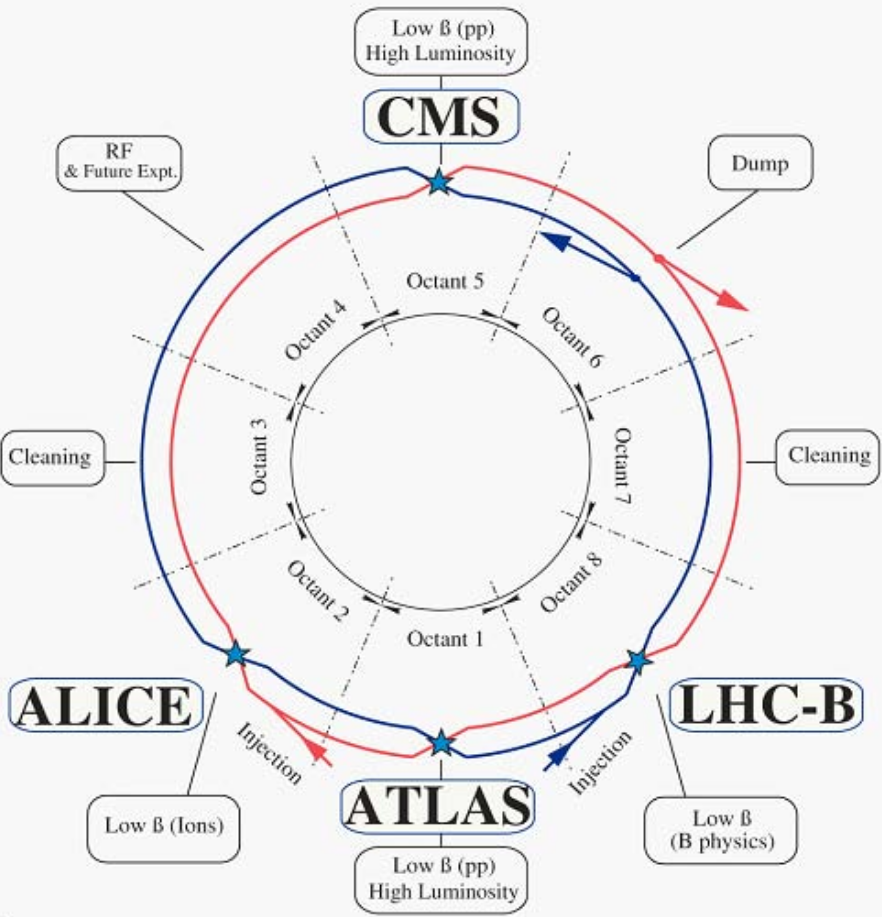
\includegraphics{Detector/Figures/LHC.png}}

\caption{Schematic of the LHC ring showing the two beams as well as the four major experiments. It also shows the injection points as well as the cleaning point and the beam dump. \cite{1748-0221-3-08-S08001}
  \label{fig:det_LHC}}
  \end{center}
\end{figure}

The instantaneous luminosity $\mathcal{L}$ is a measure for the rate of delivered collisions.
It is related to the rate of events $\dot N$ of a process $k$ through the cross section $\sigma_k$:

\begin{equation}
\dot N_k = \mathcal{L} \cdot \sigma_k.
\end{equation}

The luminosity itself can be calculated from the beam properties as given in Equation \ref{}.

\begin{equation}
\mathcal{L} = \frac{N_b \cdot N_p^2 \cdot v}{A}
\end{equation}

Here, $N_b$ stands for the number of bunches, $N_p$ for the number of protons per bunch and $A$ for the profile of the two beams at the interaction.
\todo{different Formula ??}

This analysis uses \lumiv of data taken at a center of mass energy of $\sqrt{s} = 13 \TeV$.

\section{The CMS Detector}

The CMS detector is constructed as a multi purpose detector to study particles from proton-proton, proton-lead and lead-lead collisions.
With a length of 21.6 m, a 15 m diameter it is comparatively small and dense for its weigth of 14000 tons.

The detector is build of multiple radial layers ("onion structure") and split into the barrel region in the middle and two endcaps closing up the detector structure as shown in the overview in Figure \ref{fig:det_CMS}.
The innermost part of the detector is the tracker, followed by the electromagnetic and then the hadronic calorimeter.
These parts of the detector are surrounded by the superconducting solonoid. The muon system is the last part of the detector and situated outside the solonoid. It is interleaved with the return yoke of the magnet.

\begin{figure}[htbp!]
  \begin{center}
      \resizebox{0.89 \textwidth}{!}{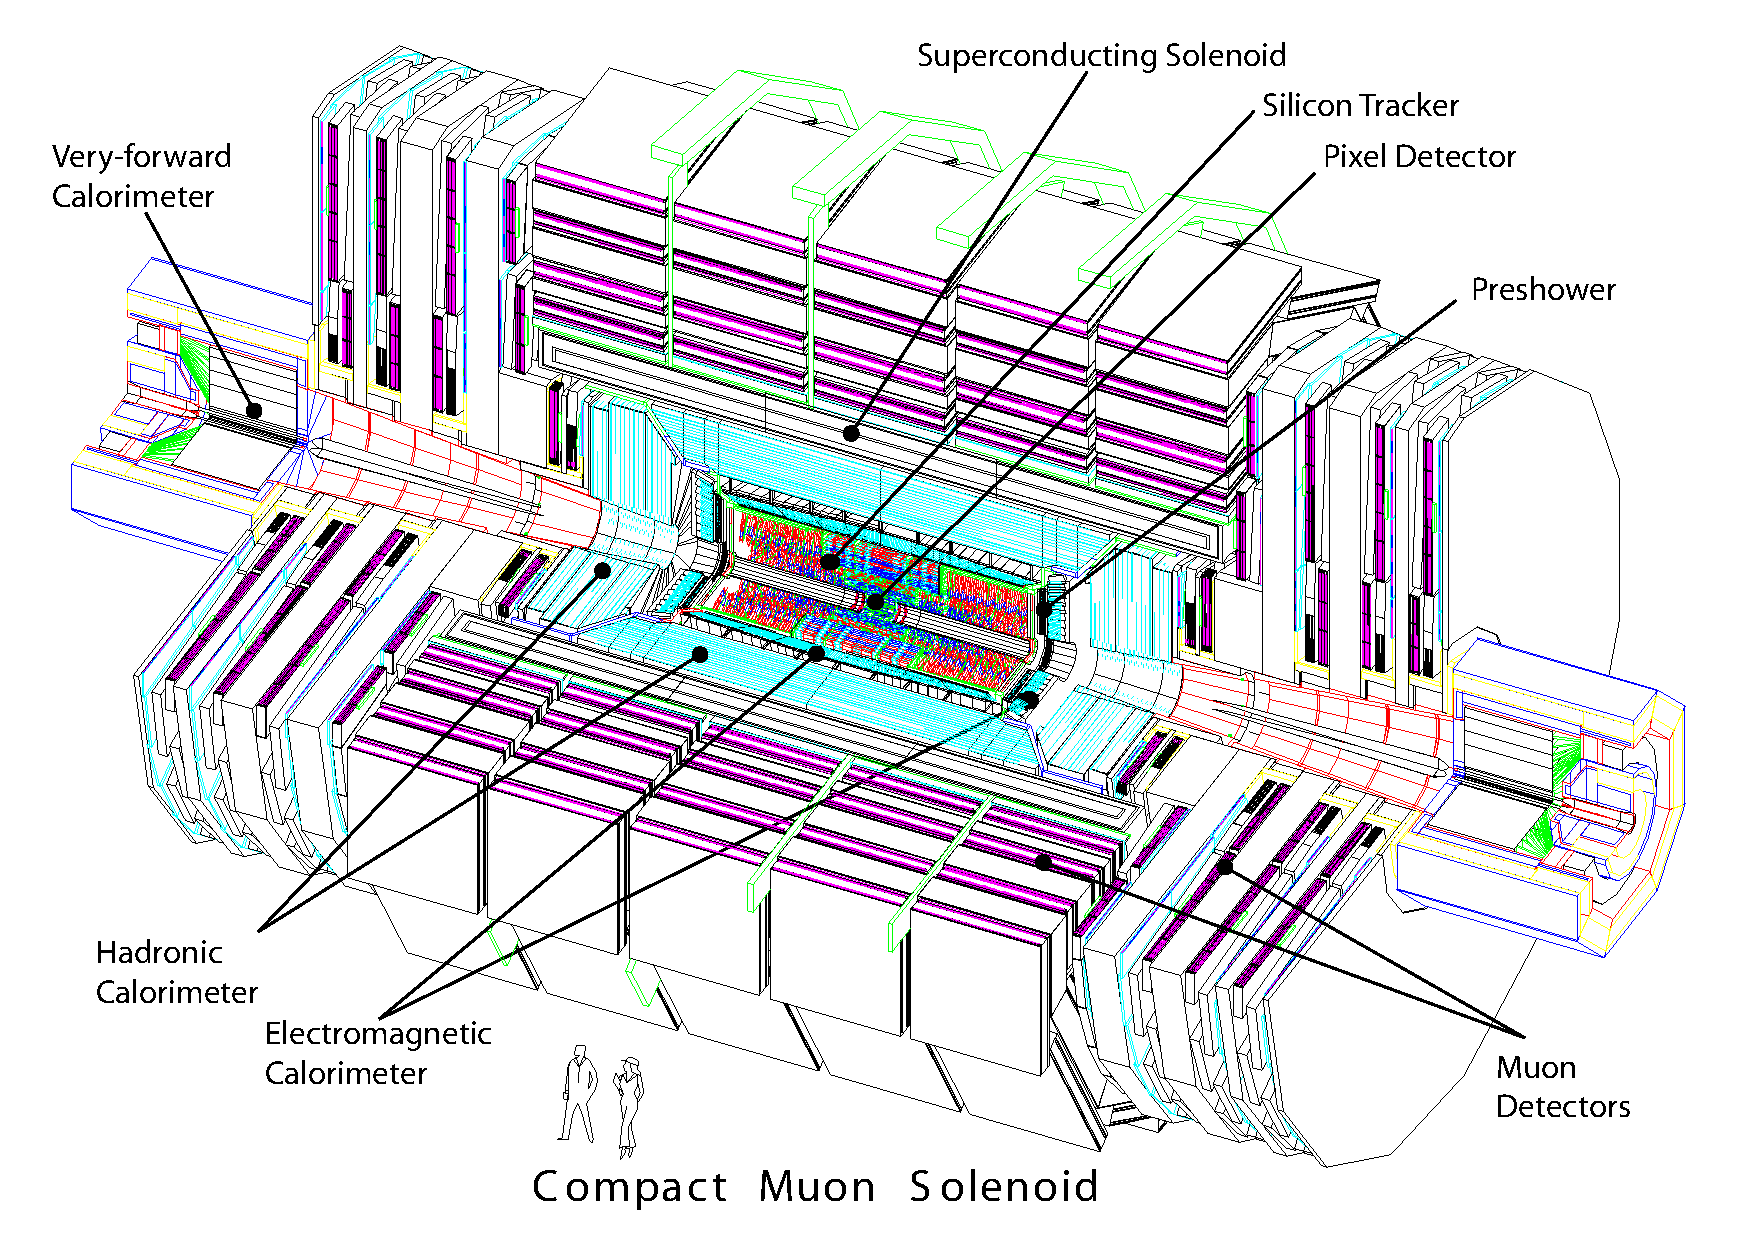
\includegraphics{Detector/Figures/cms_complete_labelled}}

\caption{The CMS detector and its relevant subsystems. \cite{Collaboration:1433717}
  \label{fig:det_CMS}}
  \end{center}
\end{figure}


The solonoid provides a magnetic field of 3.8 T for the inner part of the detector (the tracker and calorimeters) and a field of about 2 T in the muon system.
A total energy of 2.6 GJ \todo{check number} is stored in 2168 loops of superconducting cables.
This strong magnetic field leads to strongly bend tracks for charged particles allowing a precise measurement of their momenta. 
The tracks of particles outside the magnet are bend in the opposite direction of those in the inner part.

The detector is described in a right-handed coordinate system with the origin in the interaction point.
The z-axis points in the direction of the beam, the y-axis points vertically upwards and the x-axis radially points towards the center of the LHC ring.
The $\varphi$ angle is defined in the x-y plane, while the angle $\theta$ is defined in the y-z plane. Instead of $\theta$ the pseudorapidity $\eta$ is used by convention:

\begin{equation}
\eta = -\ln{\tan{\frac{\theta}{2}}}
\end{equation}

The subdequent sections describe the different parts of the detector including the triggering system that is used to select the collisions for which data is stored for analysis.

\todo{add citations}

\subsection{The Tracking System}

The tracking system \cite{Bayatian:922757} is designed to measure both tracks and vertices with a high precision.
This requires high granularity and in the LHC environment a fast response.

The tracking system is comprised of two parts: the inner one with pixels, the outer one with strips.
Its structure in the barrel as well as the endcaps is shown in Figure \ref{fig:det_Tracker}.

\begin{figure}[htbp!]
  \begin{center}
      \resizebox{0.75 \textwidth}{!}{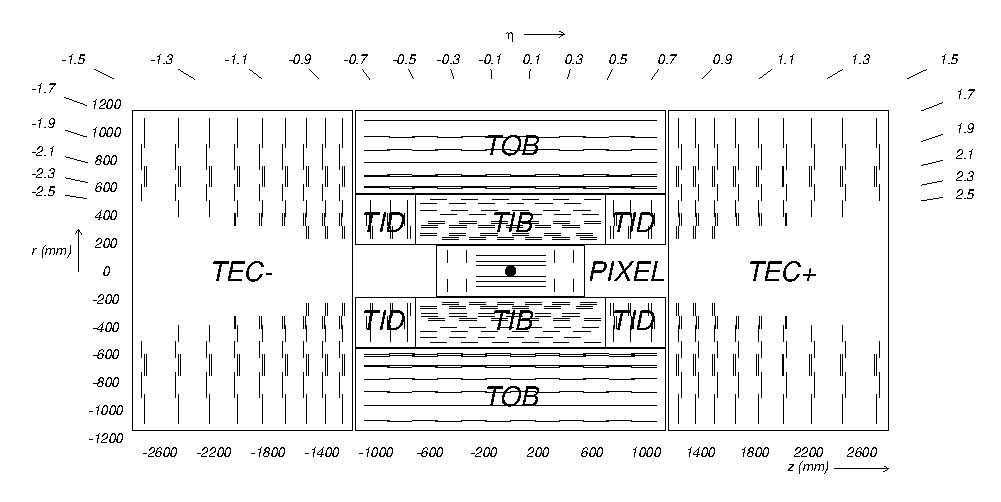
\includegraphics{Detector/Figures/TrackerLayout}}

\caption{The Tracking system of the CMS detector in the barrel and endcap regions. The sketch shows the pixel as well as the strip tracker. The strip tracker consists of the inner barrel (TIB), outer barrel (TOB), inner disks (TID) and endcaps (TEC) parts \cite{Dominguez:1481838}.
  \label{fig:det_Tracker}}
  \end{center}
\end{figure}



The first pixel layer is located at a radius of $4.4 \; \si{\centi \meter}$ in the barrel and at $34.5 \; \si{\centi \meter}$ in the endcaps.
Both parts cover a range of $|\eta| < 2.5$.
The barrel region includes three layer of pixel detectors and ten layers of strip detectors, while the endcap includes two layers of pixels and twelve layers of strips.
The 66 milion pixels measure $150 \times 100 \; \si{\micro \meter}$. The 9.6 million strips have a width of $80-180 \; \si{\micro \meter}$, together with the pixel that allows to separate even closely spaced
particle trajectories.
The position of each tracker part is precisely known from alignment analyses using cosmic muon data \cite{Chatrchyan:2014wfa}.

The momenta of charged hadrons with a $\pt < 20 \GeV$ are measured with a resolution of $1\; \%$ at normal incidence \cite{Sirunyan:2017ulk}. The relative resolution decreases for higher \pt reaching a resolution corresponding to 
the energy resolution of the calorimeter at several hundred \GeV. Since high \pt partons usually produce multiple charged hadrons of lower \pt through fragmentation the tracker can still contribute significantly 
to the measurement of high \pt jets.

\subsection{The Electromagnetic Calorimeter}

The electromagnetic calorimeter (ECAL)\cite{Bayatian:922757} measures the energy of electrons and photons that produce showers in the ECAL.
These electromagnetic showers should be contained within the ECAL. Additionally, the granularity of the ECAL should allow to separate the signals from separate particles.
A sketch of the structure of the ECAL is shown in Figure \ref{fig:det_ECAL}.

\begin{figure}[htbp!]
  \begin{center}
      \resizebox{0.75 \textwidth}{!}{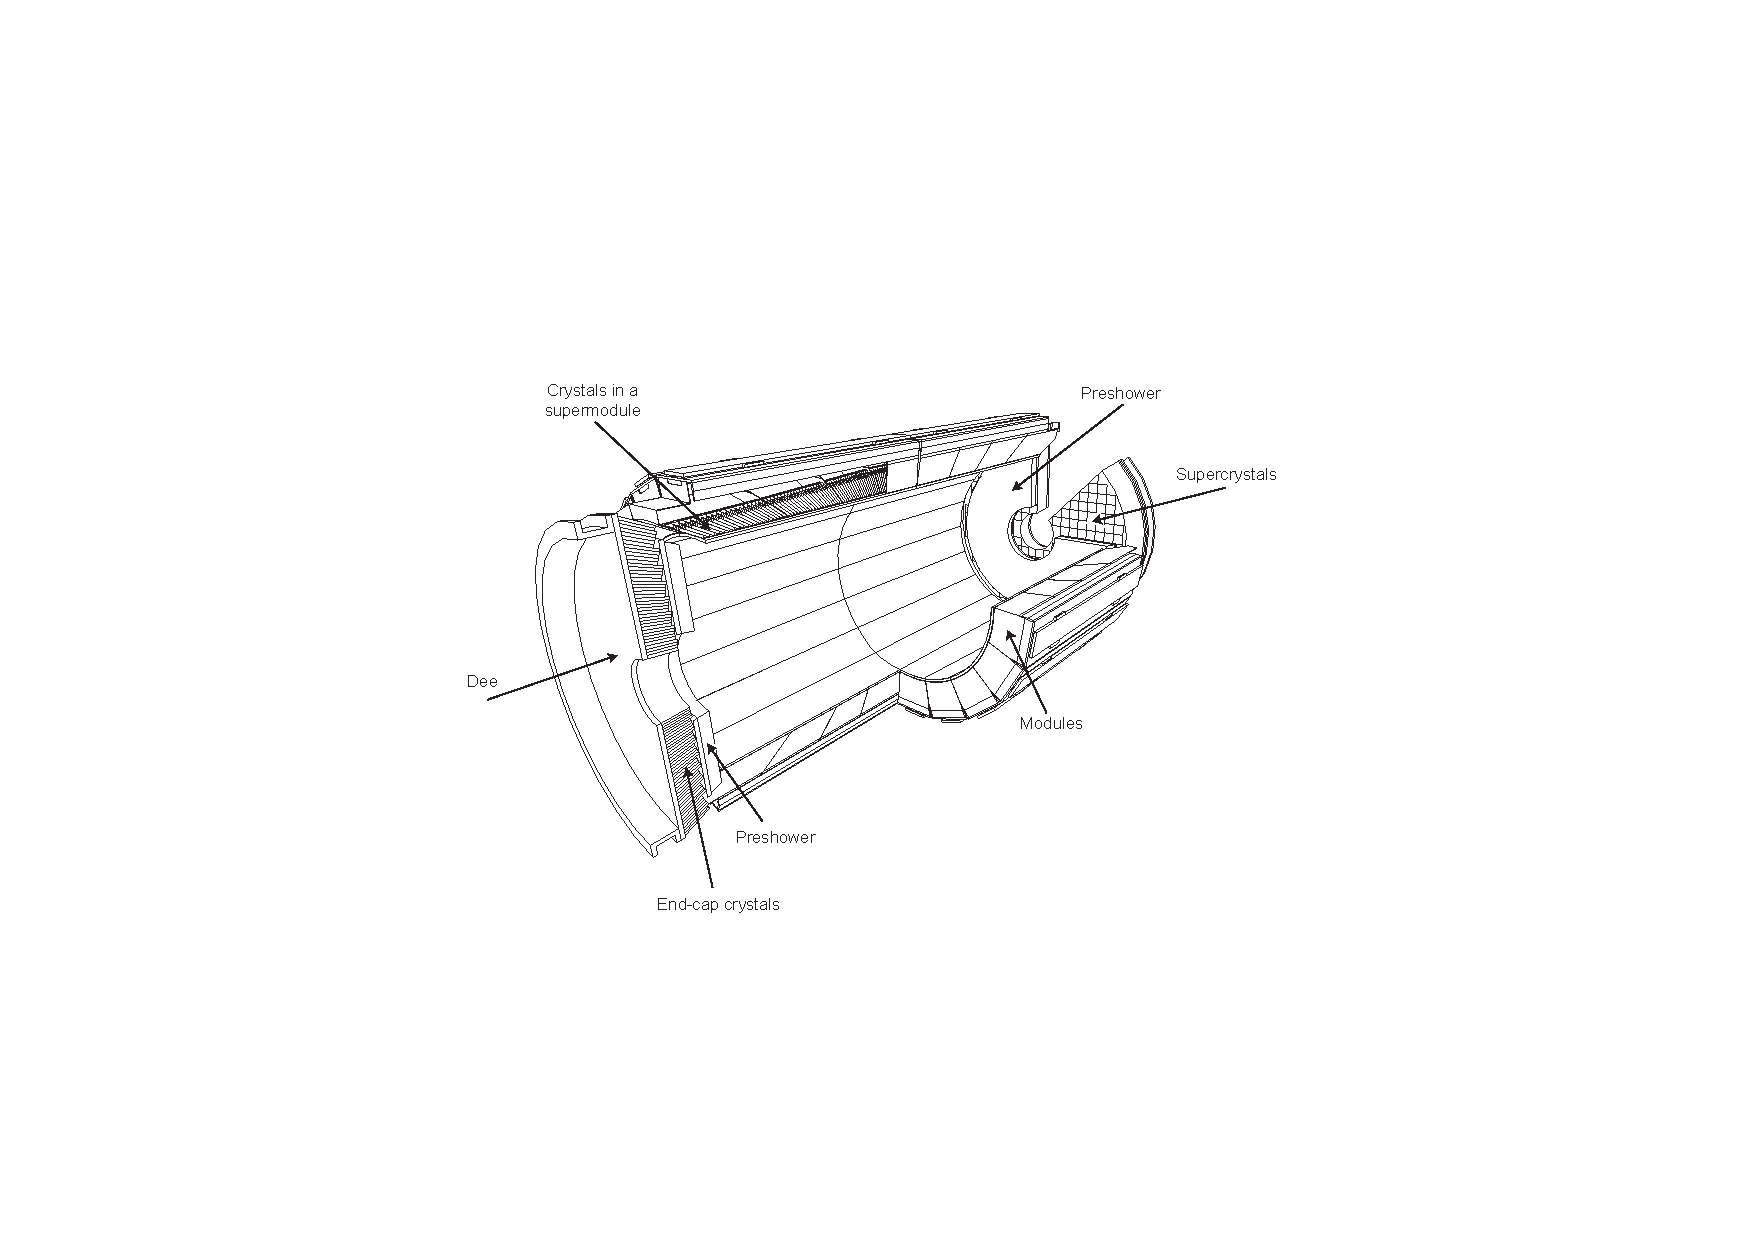
\includegraphics{Detector/Figures/ECAL}}

\caption{A sketch of the Electromagnetic Calorimeter showing the structure in the barrel and the endcaps as well as the preshower detectors. \cite{Chatrchyan:2009qm}.
  \label{fig:det_ECAL}}
  \end{center}
\end{figure}

The ECAL is made of lead tungstate with the barrel region covering about $|\eta| < 1.5$ and the endcaps covering $1.5 < |\eta|<3.0$. The crystals are $23 (22) \; \si{\centi \meter}$ in the barrel (endcap) corresponding to about 26(25) radiation lengths.
For electrons and photons up to an energy of $1 \TeV$ more than $98 \; \%$ of the energy of each particle is completely contained in the ECAL.
The crystal also correspond to roughly one interaction length, so approximately two thirds of the hadrons start their shower in the ECAL.

The front of the crystals have a size of $2.2 \time 2.2 \si{\centi \meter \squared}$ in the barrel and $2.2 \time 2.2 \si{\centi \meter \squared}$ in the endcaps. This size corresponds to the Moliere radius of the 
lead tungstate of $2.2 \si{\centi \meter}$.
The electronic noise in the ECAL is measured to be about $40 \MeV$ per crystal in the barrel and about $100 \MeV$ in the endcaps.

The energy resolution for an electron measured in the ECAL can be parameterized depending on the electron energy as follows \cite{Sirunyan:2017ulk}:

\begin{equation}
\frac{\sigma}{\mathrm{E}} = \frac{2.8\%}{\sqrt{\mathrm{E}/\GeV}} \oplus \frac{12\%}{\mathrm{E} / \GeV} \oplus 0.3\%.
\end{equation}

Photons in jets have a typical energy range of $1-50 \GeV$ where the resolution of the ECAL is excellent.

The so called preshower detector is situated in front of the two ECAL disks in the endcaps.
The preshower contains two layers: The first is a lead radiation followed by silicon strip sensors,
The detector has a much higher granularity then the ECAL allowing to measure the initial position of a shower from an electron or photon with a high precision.
The purpose of the preshower is to discriminate  between neutral pions decaying into two photons and prompt single photons.
Additionally a coincidence between ECAL and preshower can be used to identify electrons and photons.
The performance of the preshower is degraded through a large numbers of neutral pions resulting from hadrons interacting with the tracker material.

\subsection{The Hadronic Calorimeter}

The hadronic calorimeter (HCAL)\cite{Bayatian:922757} is a sampling calorimeter consisting of layers of brass absorbers and plastic scintillators.
It should measure the energy of hadronic showers with a high precision. Additionally it should prevent the hadronic shower of leaking into the muon system.
In the barrel it covers a range of $|\eta|< 1.3$ with a corresponding endcap coverafe of $1.3 <|\eta|< 3.0$ in the endcap.
In the barrel its about six interaction lengths thick at normal incidence, increasing to over ten interaction lengths.
The whole HCAL is shown as a sketch in Figure \ref{fig:det_HCAL}.



\begin{figure}[htbp!]
  \begin{center}
      \resizebox{0.75 \textwidth}{!}{\includegraphics{Detector/Figures/hcaldisplay.eps}}

\caption{A quarterly schematic of the hadronic calorimeter showing the HCAL in the barrel(HB) and the endcaps(HE) , the outer HCAL (HO) and the forward HCAL (HF)  \cite{2010JInst...5T3014C}.
  \label{fig:det_HCAL}}
  \end{center}
\end{figure}



The outer hadronic calorimeter (HO) is situated outside the solenoid coil, increasing the interaction length as an additional absorber.
In the very central region the interaction length is further increased by additional layers of steel.
Including the ECAL the total calorimeter system has a thickness corresponding to a minimum of about twelve interaction lengths in the barrel and 10 interaction lengths in the endcaps.
The individual towers of the ECAL have a cross section of $\Delta \eta \times \Delta \varphi = 0.087 \times 0.087$ in the central region of $|\eta|< 1.6$ and a cross section of $\Delta \eta \times \Delta \varphi = 0.017 \times 0.017$
in the more forward region.

The electronic noise is measured to be about $200 \MeV$ per tower\cite{Sirunyan:2017ulk}.
The combined energy resolution for ECAL and HCAL has been measured with a pion beam as 

\begin{equation}
\frac{\sigma}{\mathrm{E}} = \frac{110\%}{\sqrt{\mathrm{E}/\GeV}} \oplus 9\%.
\end{equation}

The hadron forward calorimeter (HF) is positioned on both sides of the detector at a distance of $11 \; \si{\meter}$ from the interaction point.
It covers a region of up to $|\eta| \approx 5$. It consists of steel absorbers and quartz fibres of two different lengths. The long quartz fibres correspond to roughly ten interaction lengths. The difference in the signal from the short and the long fibres is used to estimate the hadronic and electromagnetic components of the shower.

\subsection{The Muon System}

Muons with an energy in the order of \GeV are minimum ionising particles, having minimal interactions with matter.
They are generally not stopped and do not decay within the detector, so their momentum is measured through their tracks.
The purpose of the muon system as the final part of the detector is to identify muons and measure their momentum to a high precision.

The muon system \cite{Bayatian:922757} consists of four layers with three steel layers of the return yoke of the solenoid between them.
The central region is covered by drift tubes (DT) in the region of $|\eta|< 1.2$. The outer region is covered by cathode strip chambers(CSC) in the region of $0.9<|\eta|<2.4$.
Additionally resistive plate chambers (RPC) cover the range of $|\eta|<1.6$.
A sketch of the whole muon system is shown in Figure \ref{dig:det_muon}.

\begin{figure}[htbp!]
  \begin{center}
      \resizebox{0.75 \textwidth}{!}{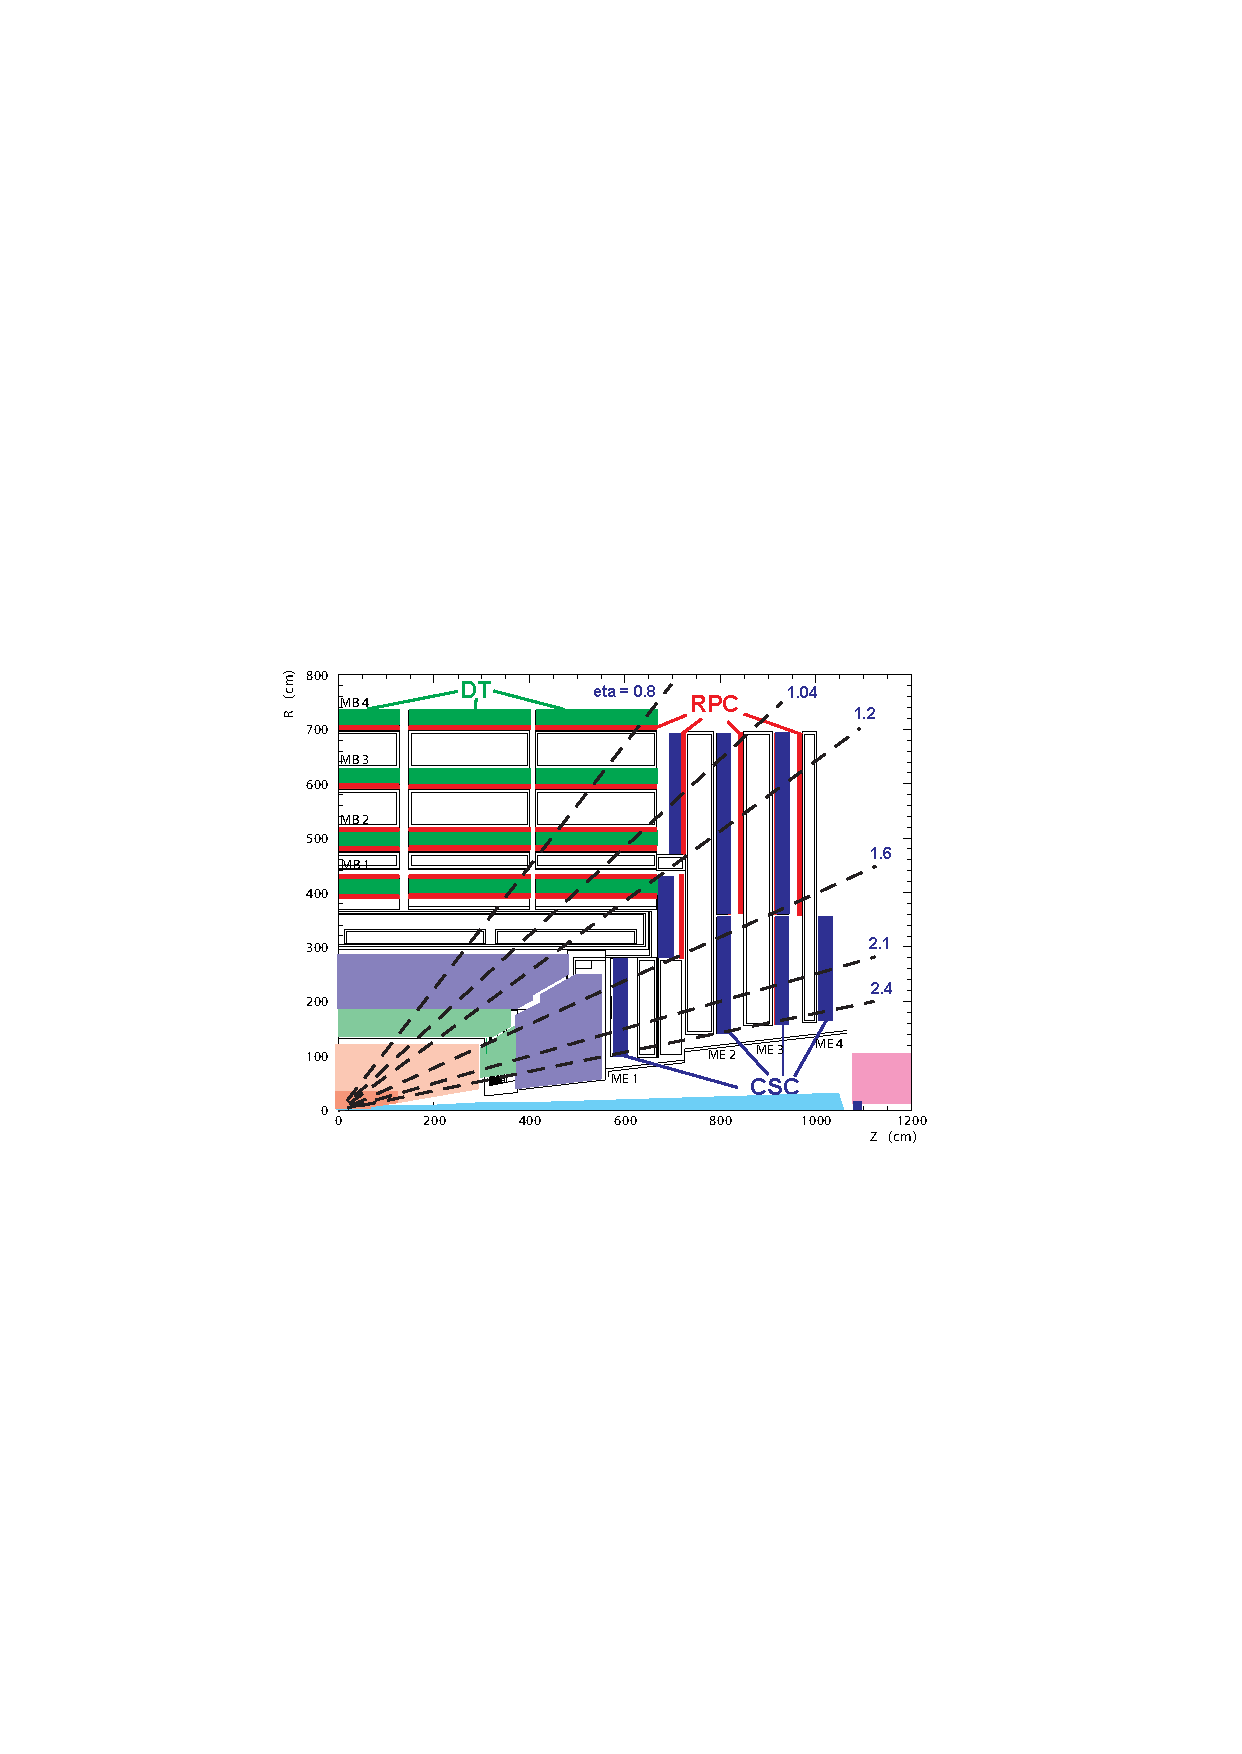
\includegraphics{Detector/Figures/Muon}}

\caption{A quarterly schematic of the muon system showing the drift tubes(DT) in the central part, the cathode strip chambers(CSC) in the outer part and the resistive plate chambers(RPC). \cite{Bayatian:922757}.
  \label{fig:det_muon}}
  \end{center}
\end{figure}

The DTs are filled with a mixture of Argon and Carbondioxide. The chambers themselves contain layers which are rotated against each other in some cases.
This allows to measure both the $\varphi$ and the $\eta$ projection of the track. The time resolution of the DTs allows them to be used for triggering.

The CSCs are positioned at a right angle with respect to the DTs. The single chambers consist of 6 gas gaps each. The two coordinates of the track are determined by radial cathode strips and perpendicular anode wires.
The spatial resolution of both the CSCs and the DTs is in the range of $100-200 \si{\micro \meter}$ depending on $\eta$.

The RPC system consists of 480 chambers. Its very high time resolution in the sub nano second range allows them to be used for triggering and the association of single muon tracks with a specific bunch crossing.

\subsection{Triggering}

The LHC delivers a collision rate of $40 \si{\mega \hertz}$. In order to record the data as it is measured by the detector this amount of events has to be reduced to a managable amount, by
only keeping those events for further study in which a relevant result is observed. A two tiered triggering system is used to reduce the final rate of events to $100 \si{\hertz}$.
First the hardware based Level-1 (L1) Trigger is used to reduce the number of events for the software based high-level trigger (HLT) \cite{Bayatyan:706847,Tapper:2013yva}.

The L1 trigger consists of programmable electronics using information from the calorimeters as well as the muon system as shown in Figure \ref{fig:det_trigger}. The tracking system is not used at this stage of triggering.
The L1 trigger is separated into the muon trigger and the calorimeter trigger. The muon trigger combines track information from the CSCs, DTs and RPCs. It uses information from the calorimeters to check the isolation of the muons.
The calorimeter trigger combines the ECAL, HCAL and HF. Besides muons algorithms targetting electrons/photons, taus, jets and the overall energy deposition in the detector are used. Requiring a muon to be contained within a jet allows to target jets originating from a b quark.
The L1 trigger has a maximal latency of $3.8 \; \si{\micro \second}$ in which a trigger decision has to be delivered to the HLT.

\begin{figure}[htbp!]
  \begin{center}
      \resizebox{0.75 \textwidth}{!}{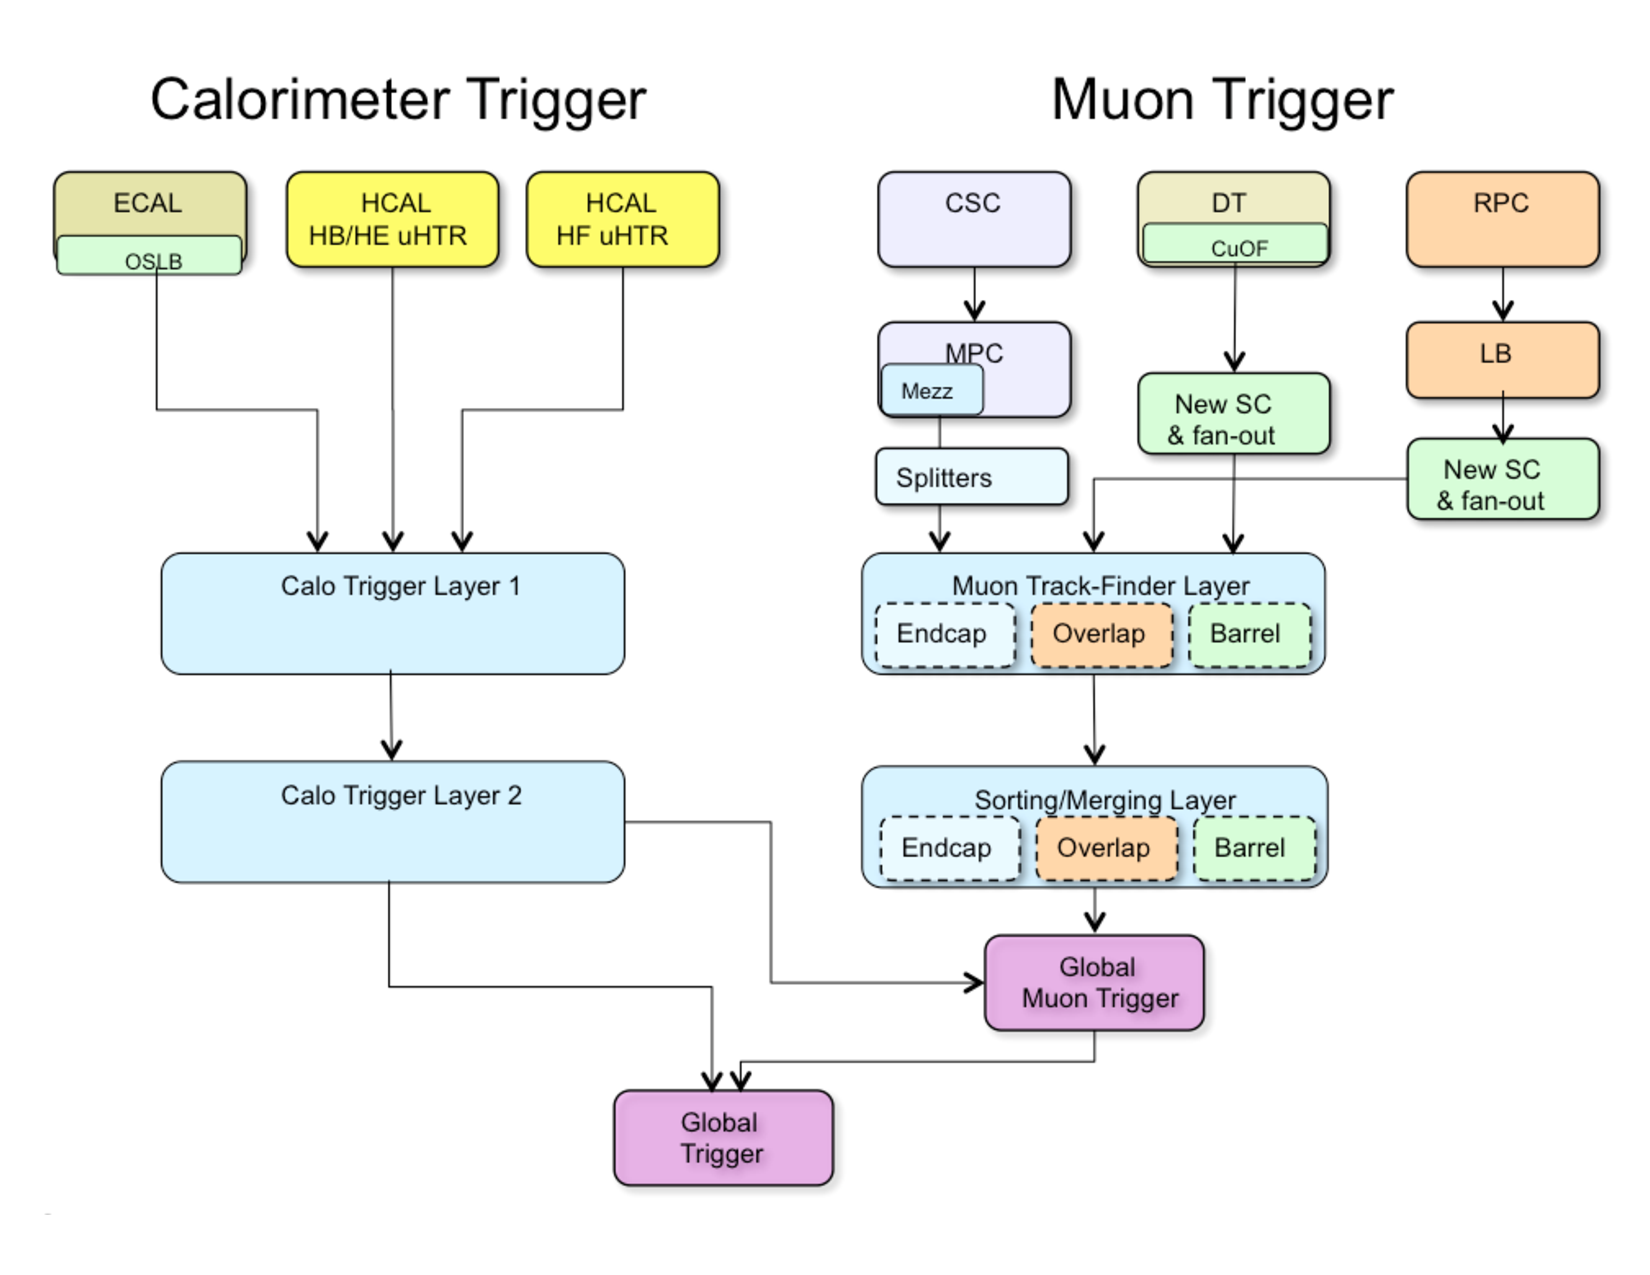
\includegraphics{Detector/Figures/Trigger}}

\caption{ Dataflow of the L1 trigger system showing the combination of information from the different subsystems \cite{Tapper:2013yva}.
  \label{fig:det_Trigger}}
  \end{center}
\end{figure}

The HLT is the second step of the triggering system. It reduces the number of events from $100 \; \si{\kilo \hertz}$ to $100 \; \si{\hertz}$.
It uses more sophisticated reconstruction techniques compared to the L1 trigger, which are generally close to the final reconstruction that is used for analysis.
The HLT starts from the L1 decision by confirming it. It then combines information from the complete detector including tracks to reconstruct the respective particle in the path.
In the end further thresholds on the kinematics, the isolation or the reconstruction quality can be required. The impact of additional soft collisions in an interaction is also mitigated in the reconstruction.
These steps are performed sequentially, if one fails the sequence is stopped. 

In order to be able to reduce the rate of certain trigger paths for both the L1 and the HLT some trigger path only consider a fraction of events. This technique is called prescaling. If a trigger path is prescaled by two it only considers every second event.

